\documentclass{beamer}

\usetheme{Warsaw}

\title{Review Guidelines}
\author{Naeem Abbasi}
\date{\today}
\institute{Institution}

\begin{document}

\begin{frame}
    \frametitle{Review Guidelines and Submission Procedure}
    \bigskip
    Welcome to the review guidelines presentation!
    
    \bigskip
    As a reviewer for ISCAS-2025, your feedback is crucial in helping us select the best papers for the conference.

    \bigskip
    Many thanks in advance!
\end{frame}

\section*{Decision Recommendation}
\begin{frame}
    \frametitle{Decision Recommendations}
    \bigskip
    We use four main categories to evaluate submissions:
    \begin{itemize}
        \item ACCEPT: Represents excellent technical work \& is well written.
        \item MARGINAL ACCEPT: Needs some changes to enhance its technical or presentation quality.
        \item MARGINAL REJECT: Content, style, examples, description of previous work or results needs major improvement.
        \item REJECT: Seriously deficient \& should not be considered for this conference.
    \end{itemize}
\bigskip
\end{frame}

\section*{Confidence Level}
\begin{frame}
    \frametitle{Confidence Level}
    \bigskip
    We use a scale from Highest to Lowest, with each level indicating increasing certainty.
    \begin{itemize}
        \item Highest: I'm extremely confident in my recommendation.
        \item High: I'm fairly certain but might have some minor doubts.
        \item Average: My confidence is moderate; I've considered both pros and cons.
        \item Low: I'm less confident; there are significant concerns or uncertainties.
        \item Lowest: I'm not at all confident; the paper doesn't meet our conference standards.
    \end{itemize}
\bigskip
\end{frame}

\section*{Relevance}
\begin{frame}
    \frametitle{Relevance}
    \bigskip
    Relevance refers to how well the paper addresses the conference topic.
    We use a scale from Excellent to Very Weak, with each level indicating increasing irrelevance.
    \begin{itemize}
        \item Excellent: The paper addresses the conference topic directly and thoroughly.
        \item Good: The paper touches on the conference topic but may not be entirely relevant.
        \item Average: The paper attempts to address the conference topic but has some gaps or limitations.
        \item Weak: The paper doesn't address the conference topic at all.
        \item Very Weak: The paper is completely off-topic and irrelevant.
    \end{itemize}
\bigskip
\end{frame}

\section*{Originality}
\begin{frame}
    \frametitle{Originality}
    \bigskip
    Originality refers to the novelty and creativity of the paper.
    We use a scale from Excellent to Very Weak, with each level indicating increasing originality.
    \begin{itemize}
        \item Excellent: The paper presents novel ideas or approaches.
        \item Good: The paper builds upon existing research but offers some new insights.
        \item Average: The paper is largely based on existing research without adding much new value.
        \item Weak: The paper lacks originality and fails to contribute to the field.
        \item Very Weak: The paper is entirely unoriginal and lacks any meaningful contribution.
    \end{itemize}
\bigskip
\end{frame}

\section*{Presentation Format}
\begin{frame}
    \frametitle{Presentation Format}
    \bigskip
    We use three main categories to determine the presentation format:
    \begin{itemize}
        \item Lecture: Best suited for longer papers with in-depth discussions.
        \item Poster: Suitable for shorter papers or those with visual components.
        \item Either: Some papers may require both formats.
    \end{itemize}
\bigskip
\end{frame}

\section*{Conclusion}
\begin{frame}
    \frametitle{Review Guidelines Summary}
    \bigskip
    To summarize:
    \begin{itemize}
        \item Decision recommendations (ACCEPT, MARGINAL ACCEPT, MARGINAL REJECT, REJECT)
        \item Confidence level (Highest to Lowest)
        \item Relevance (Excellent to Very Weak)
        \item Originality (Excellent to Very Weak)
        \item Presentation format (Lecture, Poster, Either)
    \end{itemize}
\bigskip
\end{frame}

\section*{Review Submission}
\begin{frame}
  \frametitle{Review Submission}
  \bigskip
  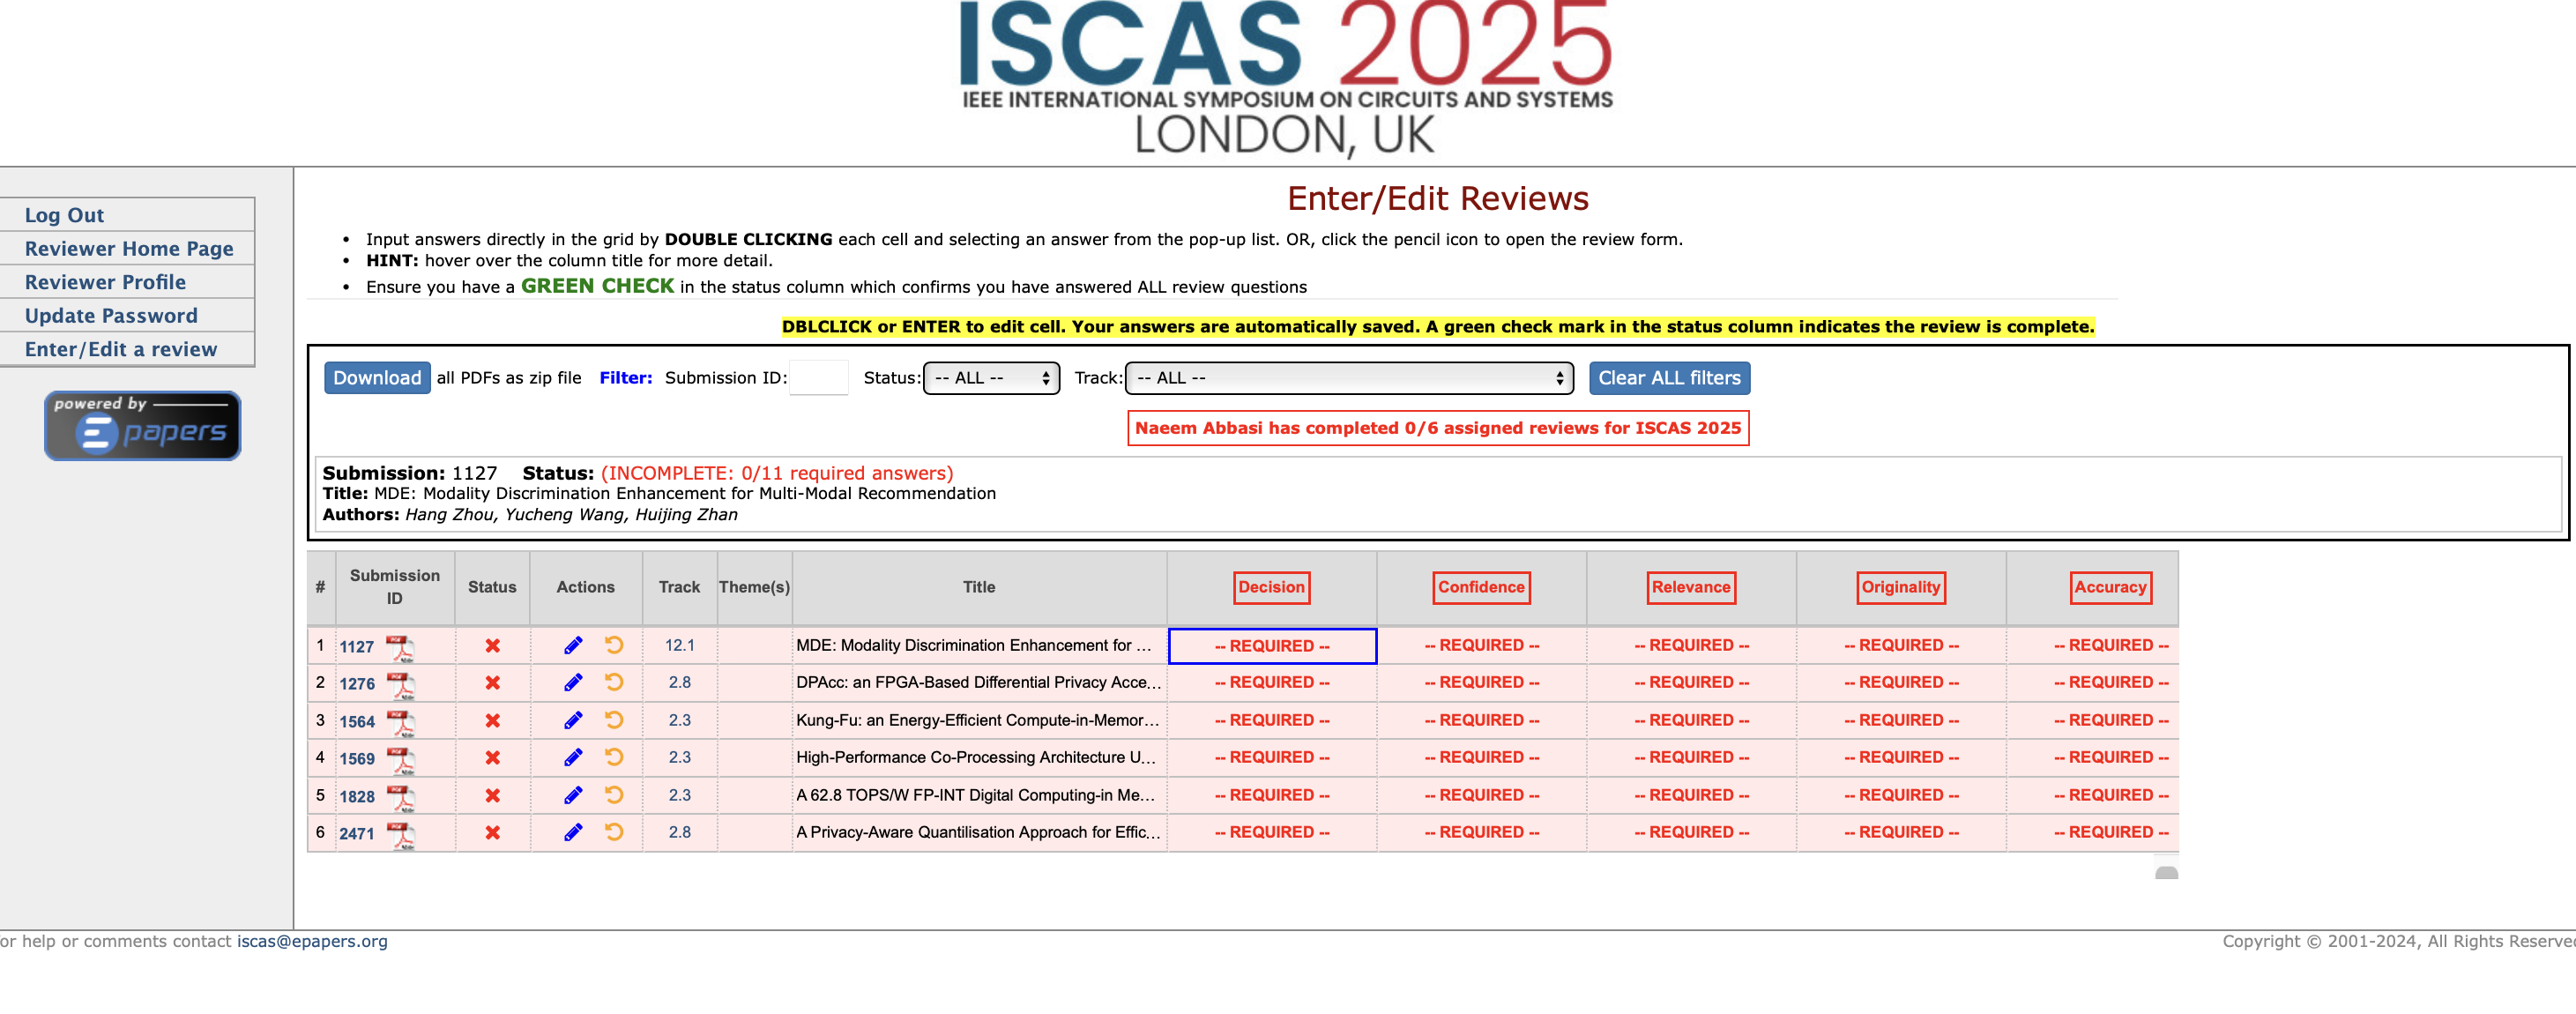
\includegraphics[width=1.0\textwidth]{ReviewSub03.png}
  \bigskip
\end{frame}


\section*{Review Submission}
\begin{frame}
  \frametitle{Review Submission}
  \bigskip
  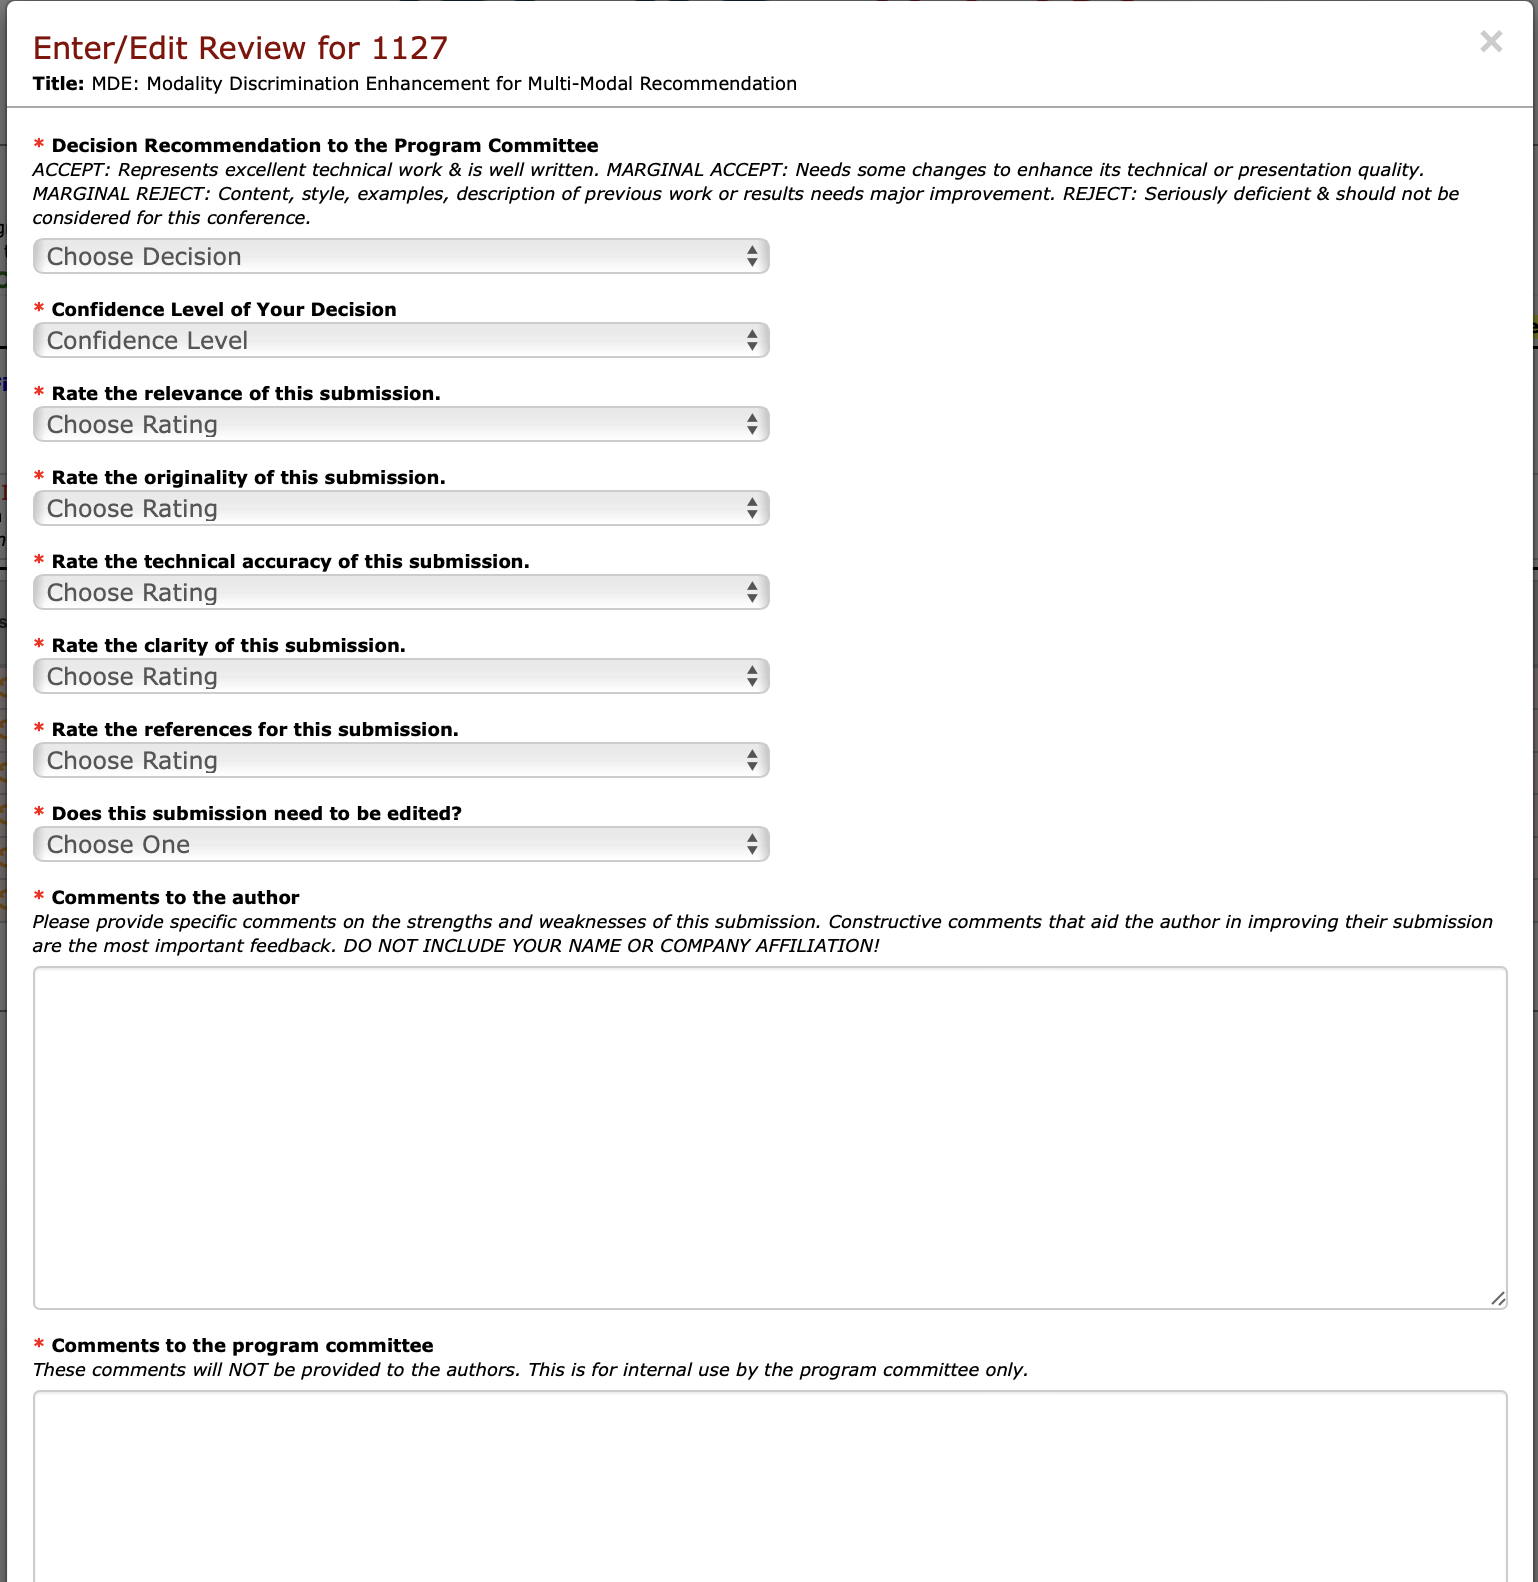
\includegraphics[width=1.0\textwidth]{ReviewSub02.png}
  \bigskip
\end{frame}




\section*{Review Submission}
\begin{frame}
  \frametitle{Review Submission}
  \bigskip
  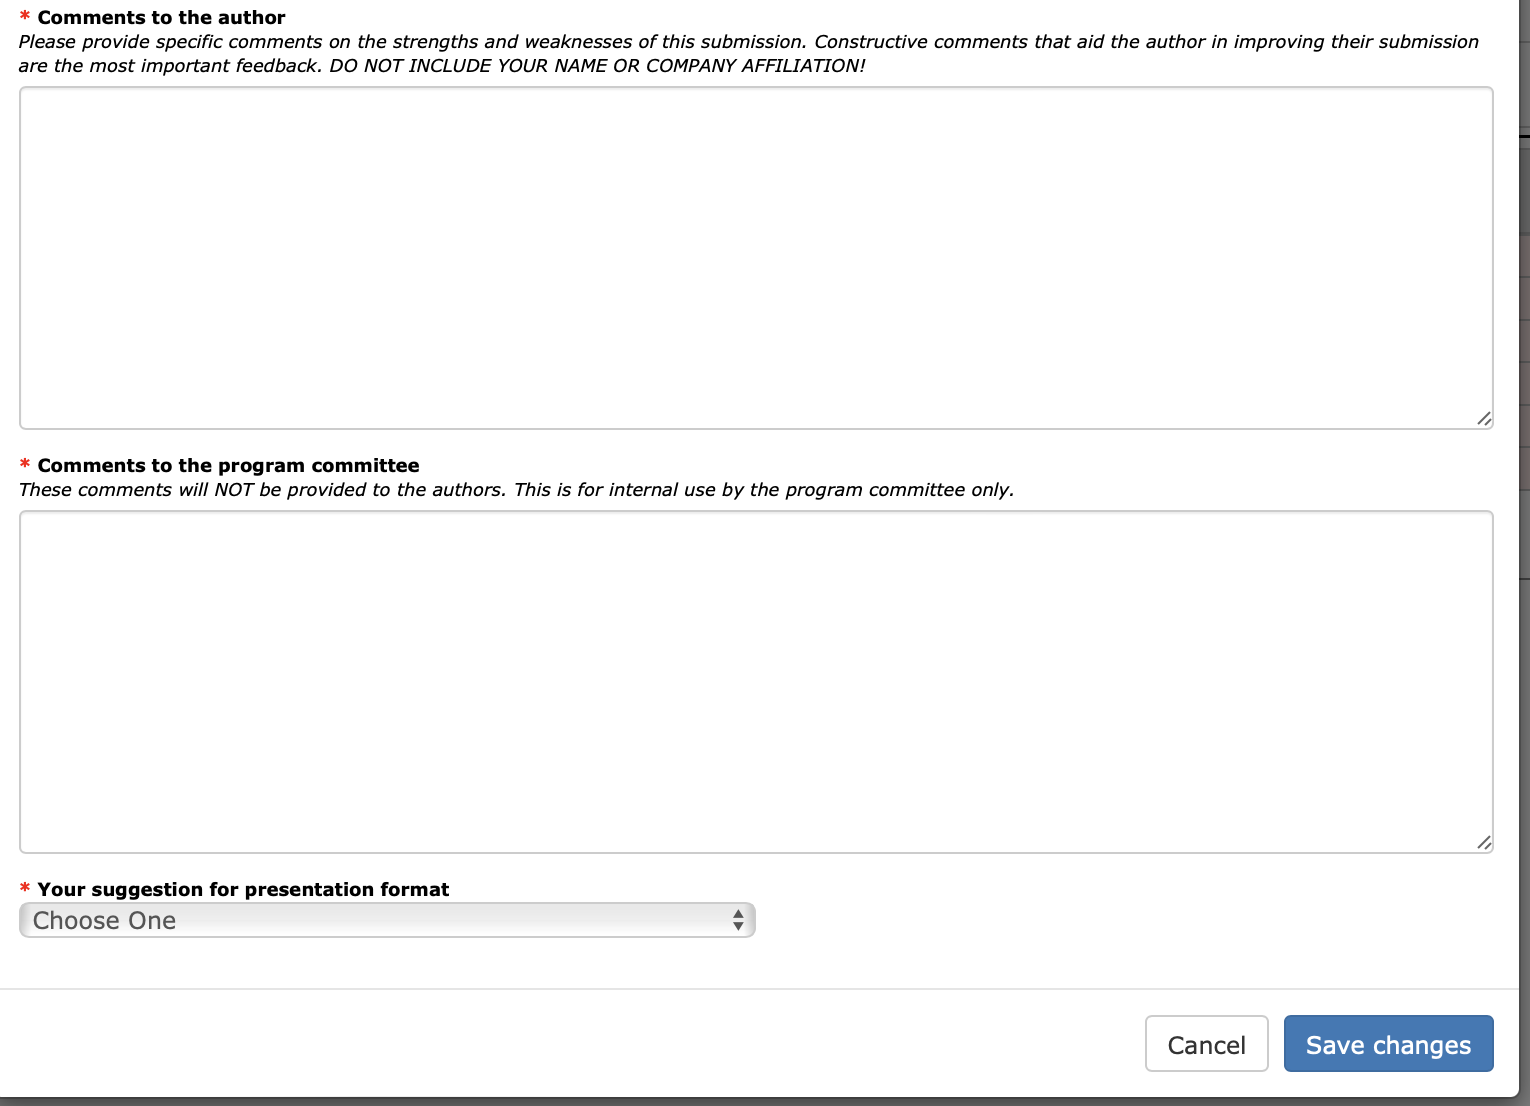
\includegraphics[width=1.0\textwidth]{ReviewSub01.png}
  \bigskip
\end{frame}

\end{document}
